% Options for packages loaded elsewhere
\PassOptionsToPackage{unicode}{hyperref}
\PassOptionsToPackage{hyphens}{url}
%
\documentclass[
]{article}
\usepackage{amsmath,amssymb}
\usepackage{iftex}
\ifPDFTeX
  \usepackage[T1]{fontenc}
  \usepackage[utf8]{inputenc}
  \usepackage{textcomp} % provide euro and other symbols
\else % if luatex or xetex
  \usepackage{unicode-math} % this also loads fontspec
  \defaultfontfeatures{Scale=MatchLowercase}
  \defaultfontfeatures[\rmfamily]{Ligatures=TeX,Scale=1}
\fi
\usepackage{lmodern}
\ifPDFTeX\else
  % xetex/luatex font selection
\fi
% Use upquote if available, for straight quotes in verbatim environments
\IfFileExists{upquote.sty}{\usepackage{upquote}}{}
\IfFileExists{microtype.sty}{% use microtype if available
  \usepackage[]{microtype}
  \UseMicrotypeSet[protrusion]{basicmath} % disable protrusion for tt fonts
}{}
\makeatletter
\@ifundefined{KOMAClassName}{% if non-KOMA class
  \IfFileExists{parskip.sty}{%
    \usepackage{parskip}
  }{% else
    \setlength{\parindent}{0pt}
    \setlength{\parskip}{6pt plus 2pt minus 1pt}}
}{% if KOMA class
  \KOMAoptions{parskip=half}}
\makeatother
\usepackage{xcolor}
\usepackage[top=2.5cm,bottom=2.8cm,left=2.8cm,right=2.5cm,margin=1in]{geometry}
\usepackage{graphicx}
\makeatletter
\def\maxwidth{\ifdim\Gin@nat@width>\linewidth\linewidth\else\Gin@nat@width\fi}
\def\maxheight{\ifdim\Gin@nat@height>\textheight\textheight\else\Gin@nat@height\fi}
\makeatother
% Scale images if necessary, so that they will not overflow the page
% margins by default, and it is still possible to overwrite the defaults
% using explicit options in \includegraphics[width, height, ...]{}
\setkeys{Gin}{width=\maxwidth,height=\maxheight,keepaspectratio}
% Set default figure placement to htbp
\makeatletter
\def\fps@figure{htbp}
\makeatother
\setlength{\emergencystretch}{3em} % prevent overfull lines
\providecommand{\tightlist}{%
  \setlength{\itemsep}{0pt}\setlength{\parskip}{0pt}}
\setcounter{secnumdepth}{5}
% preamble.tex — FINAL TESTÉ
\definecolor{mainblue}{RGB}{31, 73, 125}
\definecolor{darkblue}{RGB}{13, 43, 80}
\definecolor{lightblue}{RGB}{219, 229, 241}
\definecolor{accentred}{RGB}{178, 24, 43}
\definecolor{slategray}{RGB}{74, 85, 104}
\definecolor{smoke}{RGB}{247, 249, 252}
\definecolor{gold}{RGB}{192, 154, 47}
\definecolor{teal}{RGB}{26, 152, 80}

\usepackage{multirow}
\usepackage{makecell}
\usepackage{float}
\usepackage{wrapfig}
\usepackage{pdflscape}
\usepackage[normalem]{ulem}
\usepackage{threeparttable}
\usepackage{tikz}

\usepackage{titlesec}
\titleformat{\section}
  {\normalfont\Large\bfseries\color{mainblue}}{\thesection}{1em}{}
  [\vspace{-4pt}\color{lightblue}\rule{\linewidth}{0.8pt}]
\titleformat{\subsection}
  {\normalfont\large\bfseries\color{darkblue}}{\thesubsection}{1em}{}
\titleformat{\subsubsection}
  {\normalfont\normalsize\bfseries\color{slategray}}{\thesubsubsection}{1em}{}
\titlespacing*{\section}{0pt}{18pt}{8pt}
\titlespacing*{\subsection}{0pt}{12pt}{4pt}

\usepackage{fancyhdr}
\pagestyle{fancy}
\fancyhf{}
\fancyhead[L]{\small\color{slategray}\textit{Education et Alphabetisation --- Nigeria GHS W4}}
\fancyhead[R]{\small\color{slategray}\textit{ENSAE Pierre Ndiaye \textbullet{} ISE 1}}
\fancyfoot[C]{\small\thepage}
\renewcommand{\headrulewidth}{0.3pt}
\renewcommand{\footrulewidth}{0pt}

\usepackage{caption}
\captionsetup{labelfont={bf,color=mainblue},textfont={small,color=slategray},
  labelsep=period,skip=6pt}

\usepackage{setspace}
\onehalfspacing

% tcolorbox : aucun conflit avec booktabs (remplace mdframed)
\usepackage{tcolorbox}
\tcbuselibrary{skins,breakable}

\newtcolorbox{interpretbox}{
  enhanced, breakable,
  colback=lightblue!25, colframe=mainblue,
  boxrule=1.2pt, arc=4pt,
  left=12pt, right=12pt, top=9pt, bottom=9pt
}
\newtcolorbox{alertbox}{
  enhanced, breakable,
  colback=accentred!8, colframe=accentred,
  boxrule=1.2pt, arc=4pt,
  left=12pt, right=12pt, top=9pt, bottom=9pt
}
\newtcolorbox{recbox}{
  enhanced, breakable,
  colback=teal!8, colframe=teal,
  boxrule=1.2pt, arc=4pt,
  left=12pt, right=12pt, top=9pt, bottom=9pt
}
\usepackage{booktabs}
\usepackage{array}
\ifLuaTeX
  \usepackage{selnolig}  % disable illegal ligatures
\fi
\usepackage{bookmark}
\IfFileExists{xurl.sty}{\usepackage{xurl}}{} % add URL line breaks if available
\urlstyle{same}
\hypersetup{
  pdftitle={RAPPORT},
  hidelinks,
  pdfcreator={LaTeX via pandoc}}

\title{RAPPORT}
\author{}
\date{\vspace{-2.5em}}

\begin{document}
\maketitle

\begin{titlepage}
\thispagestyle{empty}
\begin{tikzpicture}[remember picture, overlay]
  \fill[mainblue!65] (current page.north west) rectangle ++(1.1cm,-\paperheight);
  \fill[mainblue!65] (current page.north east) rectangle ++(-1.1cm,-\paperheight);
  \fill[gold!70] (current page.north west) ++(1.1cm,0) rectangle ++(0.18cm,-\paperheight);
  \fill[gold!70] (current page.north east) ++(-1.1cm,0) rectangle ++(-0.18cm,-\paperheight);
\end{tikzpicture}
\centering\vspace*{0.3cm}
{\large\scshape Republique du Senegal}\\[3pt]
{\small\color{slategray} Un Peuple \textbullet{} Un But \textbullet{} Une Foi}\\[10pt]
{\small\color{slategray}* * * * * * * * * * * * * * * * * * * * * * *}\\[8pt]
{\normalsize Ministere de l'Economie, du Plan et de la Cooperation}\\[8pt]
{\small\color{slategray}* * * * * * * * * * * *}\\[6pt]
{\normalsize Agence nationale de la Statistique et de la Demographie}\\[6pt]
{\small\color{slategray}* * * * * * * * * * * *}\\[6pt]
{\normalsize Ecole nationale de la Statistique et de l'Analyse economique}\\[2pt]
{\normalsize\bfseries Pierre NDIAYE}\\[14pt]
\vspace{0.4cm}

\begin{tikzpicture}
  \node[fill=mainblue,draw=gold,line width=1.2pt,rounded corners=14pt,
    inner sep=16pt,text width=13cm,align=center] {
    {\large\bfseries\color{white}\scshape Projet Statistique sous R et Python}\\[6pt]
    {\scriptsize\color{lightblue!80} Analyse 2}
  };
\end{tikzpicture}
\vspace{0.6cm}
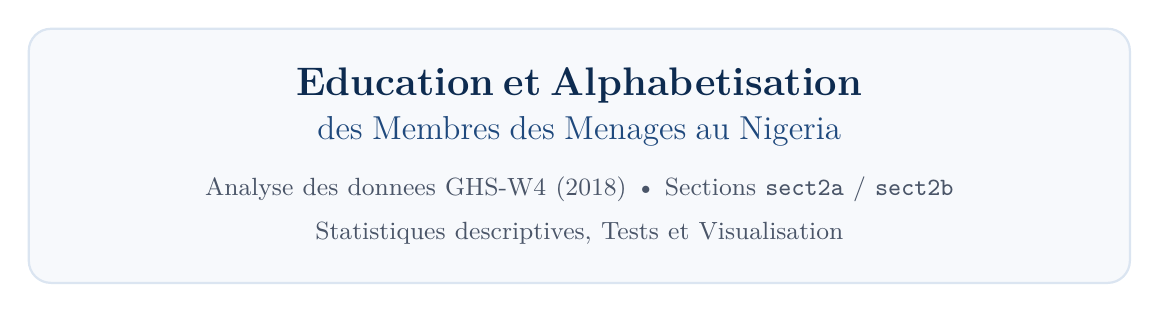
\begin{tikzpicture}
  \node[fill=smoke,draw=lightblue,line width=0.8pt,rounded corners=8pt,
    inner sep=14pt,text width=13cm,align=center] {
    {\Large\bfseries\color{darkblue} Education et Alphabetisation}\\[4pt]
    {\large\color{mainblue} des Membres des Menages au Nigeria}\\[8pt]
    {\small\color{slategray}
      Analyse des donnees GHS-W4 (2018)
      \textbullet{} Sections \texttt{sect2a} / \texttt{sect2b}}\\[4pt]
    {\small\color{slategray}
      Statistiques descriptives, Tests et Visualisation}
  };
\end{tikzpicture}
\vspace{0.8cm}
\begin{minipage}[t]{0.47\textwidth}
  \raggedright
  \underline{\textbf{\color{mainblue}Redige par :}}\\[8pt]
  \textbf{Agnangma Sanam David Landry}\\[4pt]
  \textbf{Cheikh Thioub}\\[6pt]
  {\small\color{slategray} Etudiants ISE 1 \textbullet{} 2025--2026}
\end{minipage}
\hfill
\begin{minipage}[t]{0.47\textwidth}
  \raggedleft
  \underline{\textbf{\color{mainblue}Encadre par :}}\\[8pt]
  \textbf{M. Aboubacar HEMA}\\[4pt]
  {\small\color{slategray} Ingenieur Statisticien Economiste}
\end{minipage}
\vfill

\begin{tikzpicture}
  \node[fill=mainblue!80,draw=gold,line width=1pt,rounded corners=12pt,
    inner sep=11pt,text width=5cm,align=center] {
    {\large\bfseries\color{white}\scshape Mars 2026}
  };
\end{tikzpicture}
\vspace{0.4cm}
\end{titlepage}
\cleardoublepage

{
\setcounter{tocdepth}{3}
\tableofcontents
}
\section{Introduction}\label{introduction}

Le Nigeria constitue, à bien des égards, un cas d'étude incontournable
pour l'analyse des systèmes éducatifs en Afrique subsaharienne. Première
économie du continent par son PIB nominal et première population avec
plus de 220 millions d'habitants en 2018, le pays concentre
simultanément une part significative des richesses naturelles africaines
et certaines des inégalités éducatives les plus profondes du monde
(UNESCO, 2021). L'accès à l'éducation y est profondément fracturé selon
les axes géographique (Nord/Sud, urbain/rural), de genre et de
génération --- fractures que les politiques d'universalisation scolaire
engagées depuis les années 1990, notamment l'\emph{Universal Basic
Education Act} de 2004, n'ont que partiellement résorbées.

La \emph{General Household Survey} (GHS), conduite par la Banque
Mondiale en partenariat avec le Bureau National des Statistiques
nigérian (NBS), constitue l'un des dispositifs d'enquête les plus
robustes pour documenter ces réalités à l'échelle nationale. Elle adopte
un plan de sondage stratifié à plusieurs degrés, représentatif des 36
États fédéraux et du Territoire de la Capitale Fédérale (FCT), et
collecte des informations détaillées sur les caractéristiques
démographiques, éducatives, économiques et sanitaires des membres des
ménages.

Ce rapport analyse les \textbf{niveaux d'instruction et les taux de
scolarisation} à partir de la quatrième vague du GHS Panel (GHS-W4,
2018). Il mobilise les sections éducation du questionnaire ménage ---
\texttt{sect2a} (statut scolaire actuel) et \texttt{sect2b} (niveau
atteint pour les individus ayant quitté l'école) --- complétées par les
informations sociodémographiques de \texttt{sect1} et les
caractéristiques de ménage de \texttt{secta}.

L'analyse poursuit quatre objectifs opérationnels : construire un
indicateur harmonisé de niveau d'éducation en cinq catégories ordonnées
à partir de variables partiellement redondantes et structurellement
incomplètes ; décrire la distribution nationale de cet indicateur sur la
population adulte (18 ans et plus) et sur les enfants en âge scolaire
(6--17 ans) ; identifier et quantifier les inégalités structurelles
selon le sexe, le groupe d'âge et la zone géographique ; et
cartographier les disparités inter-étatiques afin de guider un éventuel
ciblage géographique des politiques publiques.

L'échantillon final comprend \textbf{26 557 individus} répartis sur
l'ensemble du territoire national. Après traitement des valeurs
manquantes structurelles, \textbf{19 271 individus} disposent d'une
information sur leur niveau d'éducation, dont \textbf{10 345 adultes de
18 ans et plus} et \textbf{7 830 enfants âgés de 6 à 17 ans}.

\begin{center}\rule{0.5\linewidth}{0.5pt}\end{center}

\section{Données et méthodes}\label{donnuxe9es-et-muxe9thodes}

\subsection{Fichiers mobilisés}\label{fichiers-mobilisuxe9s}

L'analyse repose sur trois fichiers issus du GHS-W4 (2018). Le fichier
\texttt{sect2\_harvestw4.dta} est le fichier central : il renseigne à la
fois le statut scolaire actuel de l'individu (section \texttt{sect2a},
variables \texttt{s2aq13}, \texttt{s2aq9}, \texttt{s2aq15},
\texttt{s2aq10}) et le niveau atteint pour ceux qui ont quitté l'école
(section \texttt{sect2b}). Le fichier \texttt{sect1\_harvestw4.dta}
apporte les caractéristiques individuelles indispensables à toute
analyse bivariée, en particulier le sexe (\texttt{s1q2}) et l'âge
(\texttt{s1q4}). Enfin, \texttt{secta\_harvestw4.dta} fournit les
attributs du ménage, notamment la zone de résidence (\texttt{sector} : 1
= Urbain, 2 = Rural) et l'État d'appartenance (\texttt{state}). À noter
que la variable \texttt{sector} est également disponible directement
dans \texttt{sect2}, ce qui simplifie la jointure pour les analyses de
zone.

\subsection{\texorpdfstring{Construction de l'indicateur
\texttt{niveau\_educ}}{Construction de l'indicateur niveau\_educ}}\label{construction-de-lindicateur-niveau_educ}

L'un des défis méthodologiques centraux de cette analyse est la
construction d'un indicateur unique et cohérent de niveau d'éducation à
partir de sources multiples et partiellement redondantes. Le
questionnaire GHS distingue en effet trois situations : les individus
actuellement scolarisés (dont on connaît la classe fréquentée), les
individus ayant quitté l'école (dont on connaît le dernier niveau
atteint), et les individus n'ayant jamais été scolarisés. Ces trois
situations sont captées par des variables différentes, ce qui impose un
algorithme de codage hiérarchisé en trois passes.

La première passe traite le cas le plus simple : les individus ayant
explicitement répondu « jamais scolarisé » à la question \texttt{s2aq13}
se voient attribuer directement la catégorie \emph{Aucun}. La deuxième
passe, la plus importante en termes d'effectifs, récupère via une
fonction \texttt{coalesce} soit la classe actuellement fréquentée
(\texttt{s2aq9}), soit le dernier niveau atteint (\texttt{s2aq15}). La
troisième passe constitue un filet de sécurité : pour les individus dont
les deux variables précédentes sont manquantes, le diplôme obtenu
(\texttt{s2aq10}) permet d'inférer un niveau minimal.

Les cinq catégories finales retenues suivent la nomenclature des
systèmes scolaires anglophones d'Afrique de l'Ouest : \emph{Aucun}
(jamais scolarisé ou niveau inférieur à Primary 1), \emph{Primaire}
(Primary 1 à 6), \emph{Junior Secondary} (JSS 1--3), \emph{Senior
Secondary} (SS 1--3 ou équivalent), et \emph{Tertiaire} (NCE, OND, HND,
Licence, Master, Doctorat). Cette catégorisation est ordonnée et permet
des comparaisons statistiques non paramétriques.

\subsection{Inspection des valeurs
manquantes}\label{inspection-des-valeurs-manquantes}

Avant toute analyse, une inspection rigoureuse des valeurs manquantes
est indispensable pour évaluer les risques de biais et identifier les
éventuels problèmes de collecte. Sur les 26 557 individus de
l'échantillon joint, les variables \texttt{scolarise} (\texttt{s2aq13}),
\texttt{classe\_actuelle} (\texttt{s2aq9}) et \texttt{diplome}
(\texttt{s2aq10}) présentent toutes exactement \textbf{27,44 \%} de
valeurs manquantes, soit 7 286 individus. Cette convergence parfaite
signale un bloc de manquants structurels correspondant aux enfants trop
jeunes (nourrissons et enfants de moins de 5 ans) pour qui le module
éducation n'est pas administré dans le questionnaire. La variable
\texttt{niveau\_atteint} (\texttt{s2aq15}) affiche quant à elle
\textbf{64,95 \%} de NA, ce qui s'explique mécaniquement par la logique
du questionnaire : elle n'est renseignée que pour les individus ayant
définitivement quitté l'école, excluant donc tous les individus
actuellement scolarisés. Ces manquants sont entièrement informatifs et
ne constituent pas un problème de qualité de données. Les variables
\texttt{age} (\texttt{s1q4}) et \texttt{sexe} (\texttt{s1q2}) présentent
chacune \textbf{14,23 \%} de NA (3 780 individus), correspondant à des
membres du ménage listés mais non interviewés directement, phénomène
courant dans les enquêtes ménage à grande échelle. La variable de zone
(\texttt{sector}) est, pour sa part, complète (0 \% de NA).

Les figures ci-dessous visualisent la structure des valeurs manquantes
dans les fichiers \texttt{sect1} et \texttt{sect2}, confirmant le
caractère organisé et non aléatoire de ces absences.

\begin{figure}

{\centering 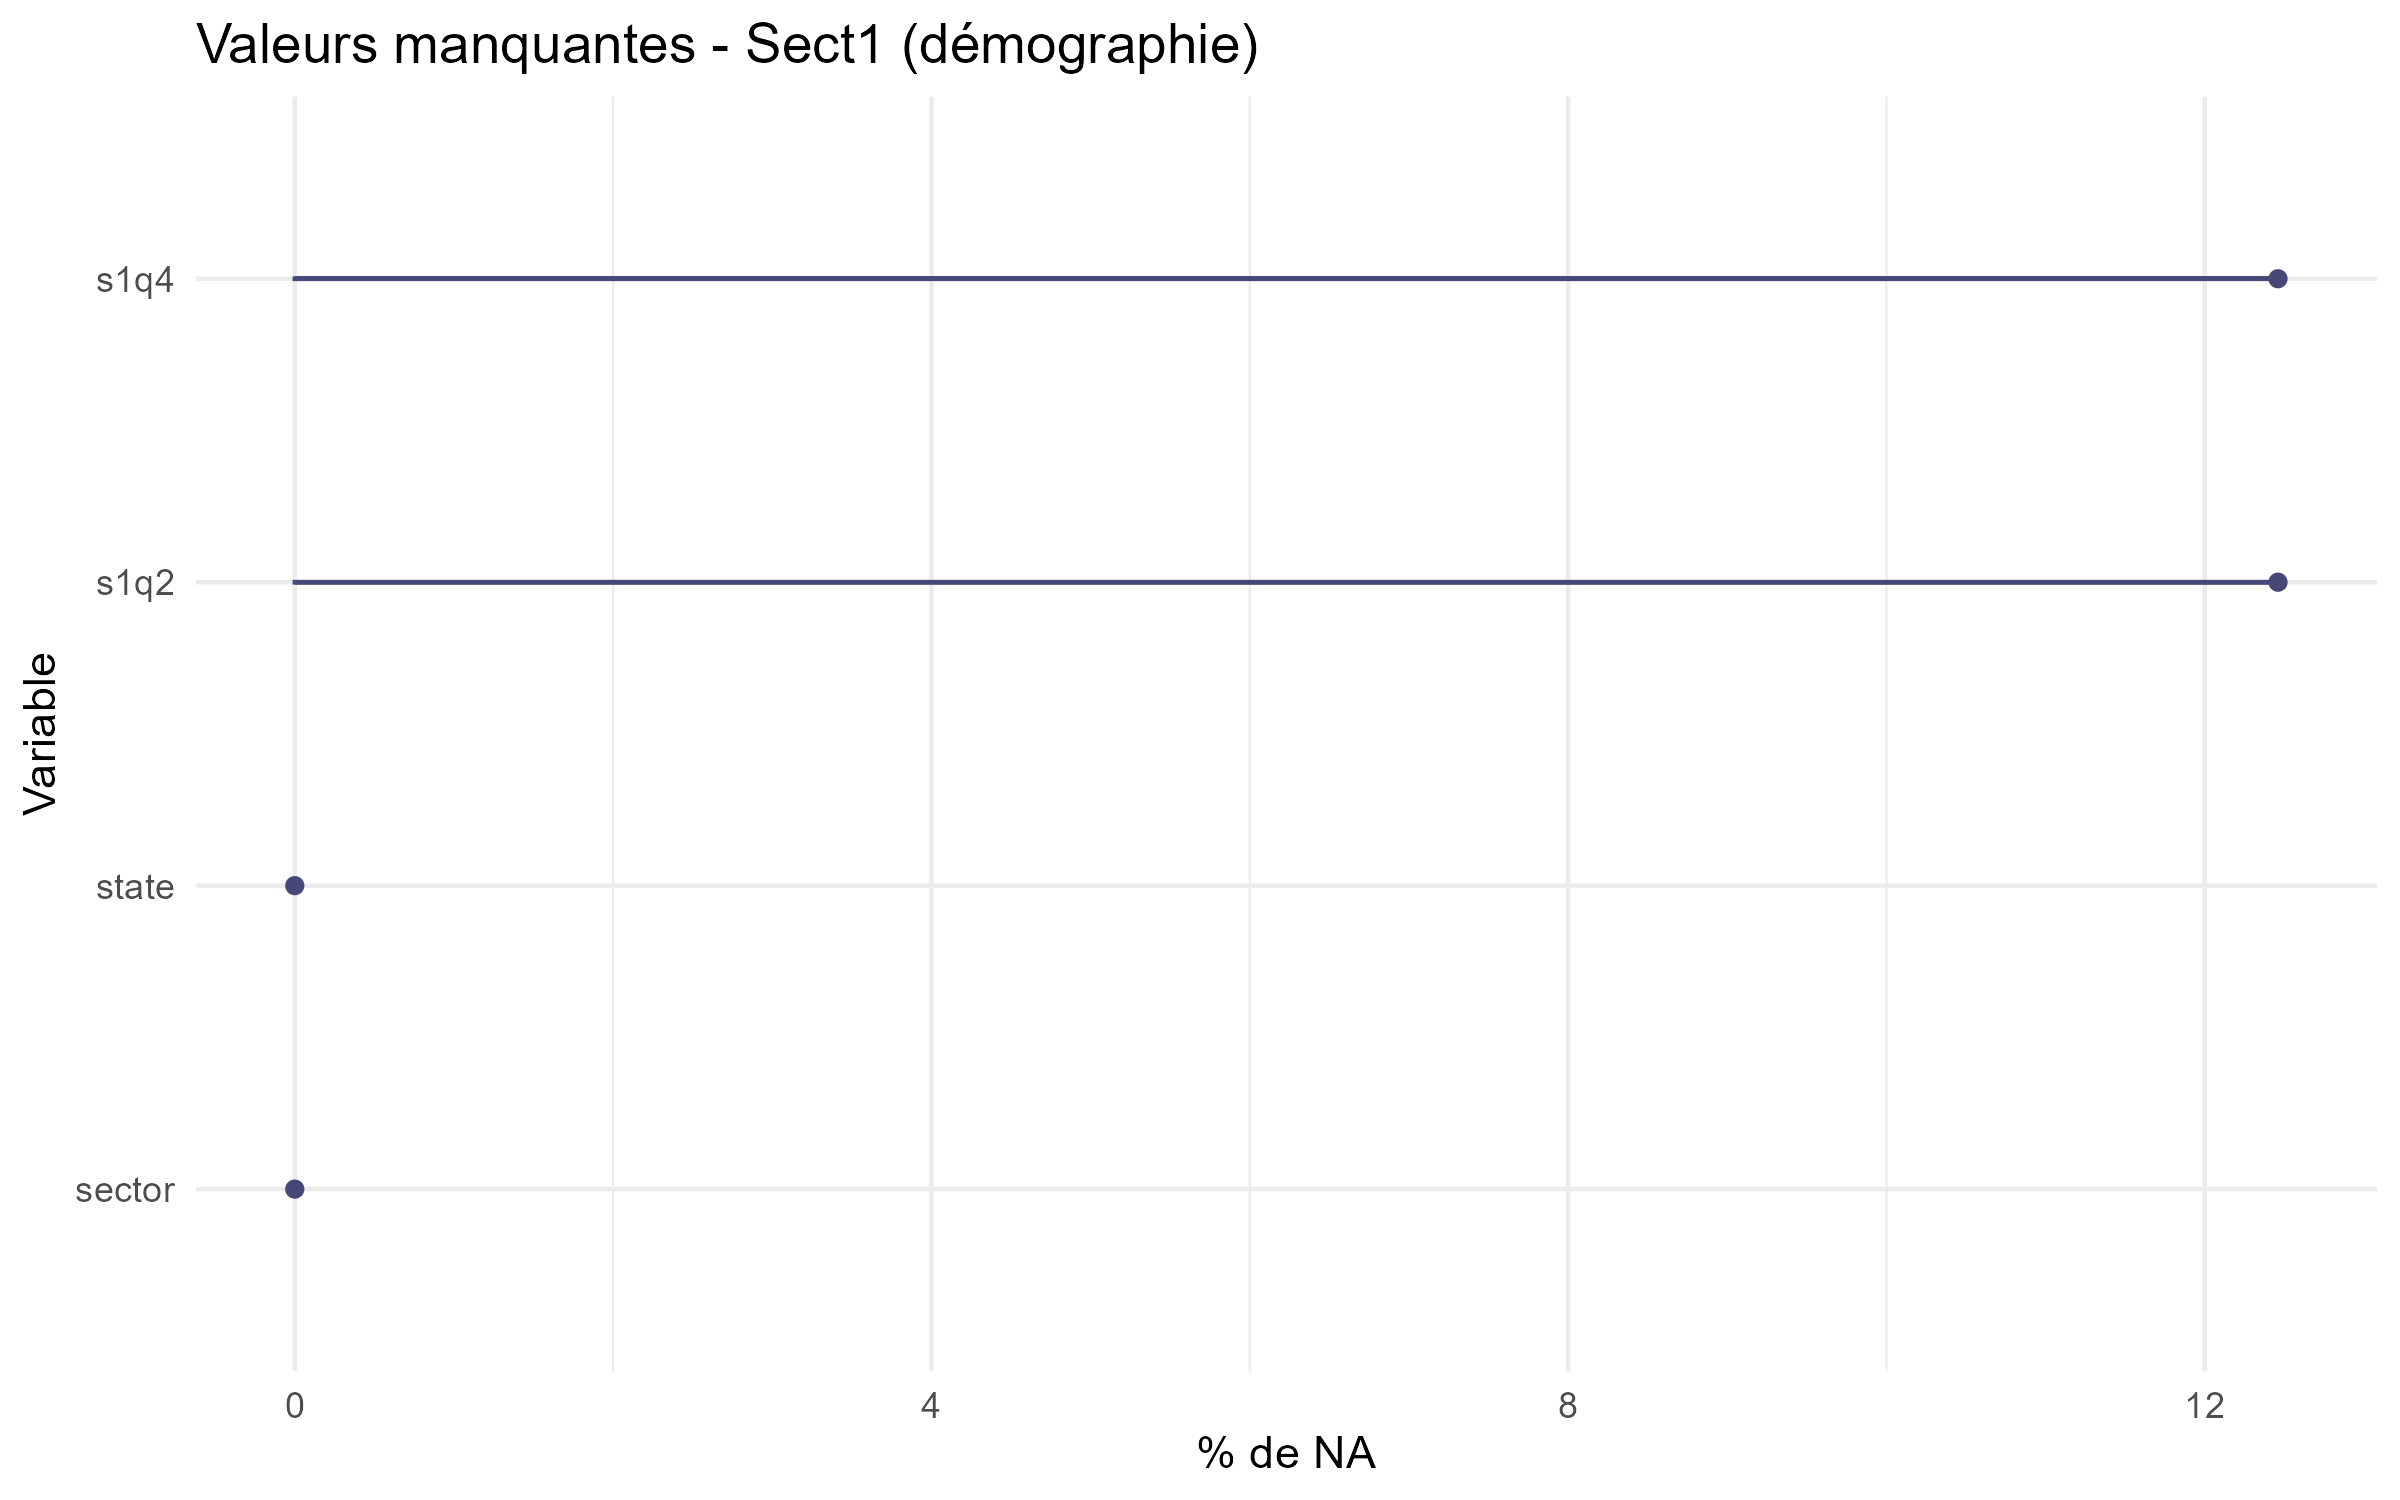
\includegraphics[width=0.95\linewidth]{../outputs/graphs/missing_sect1_tp2} 

}

\caption{Structure des valeurs manquantes dans sect1 (GHS-W4 2018) --- seules les variables avec au moins 1 NA sont representees}\label{fig:an2_fig_missing_sect1}
\end{figure}

\begin{figure}

{\centering 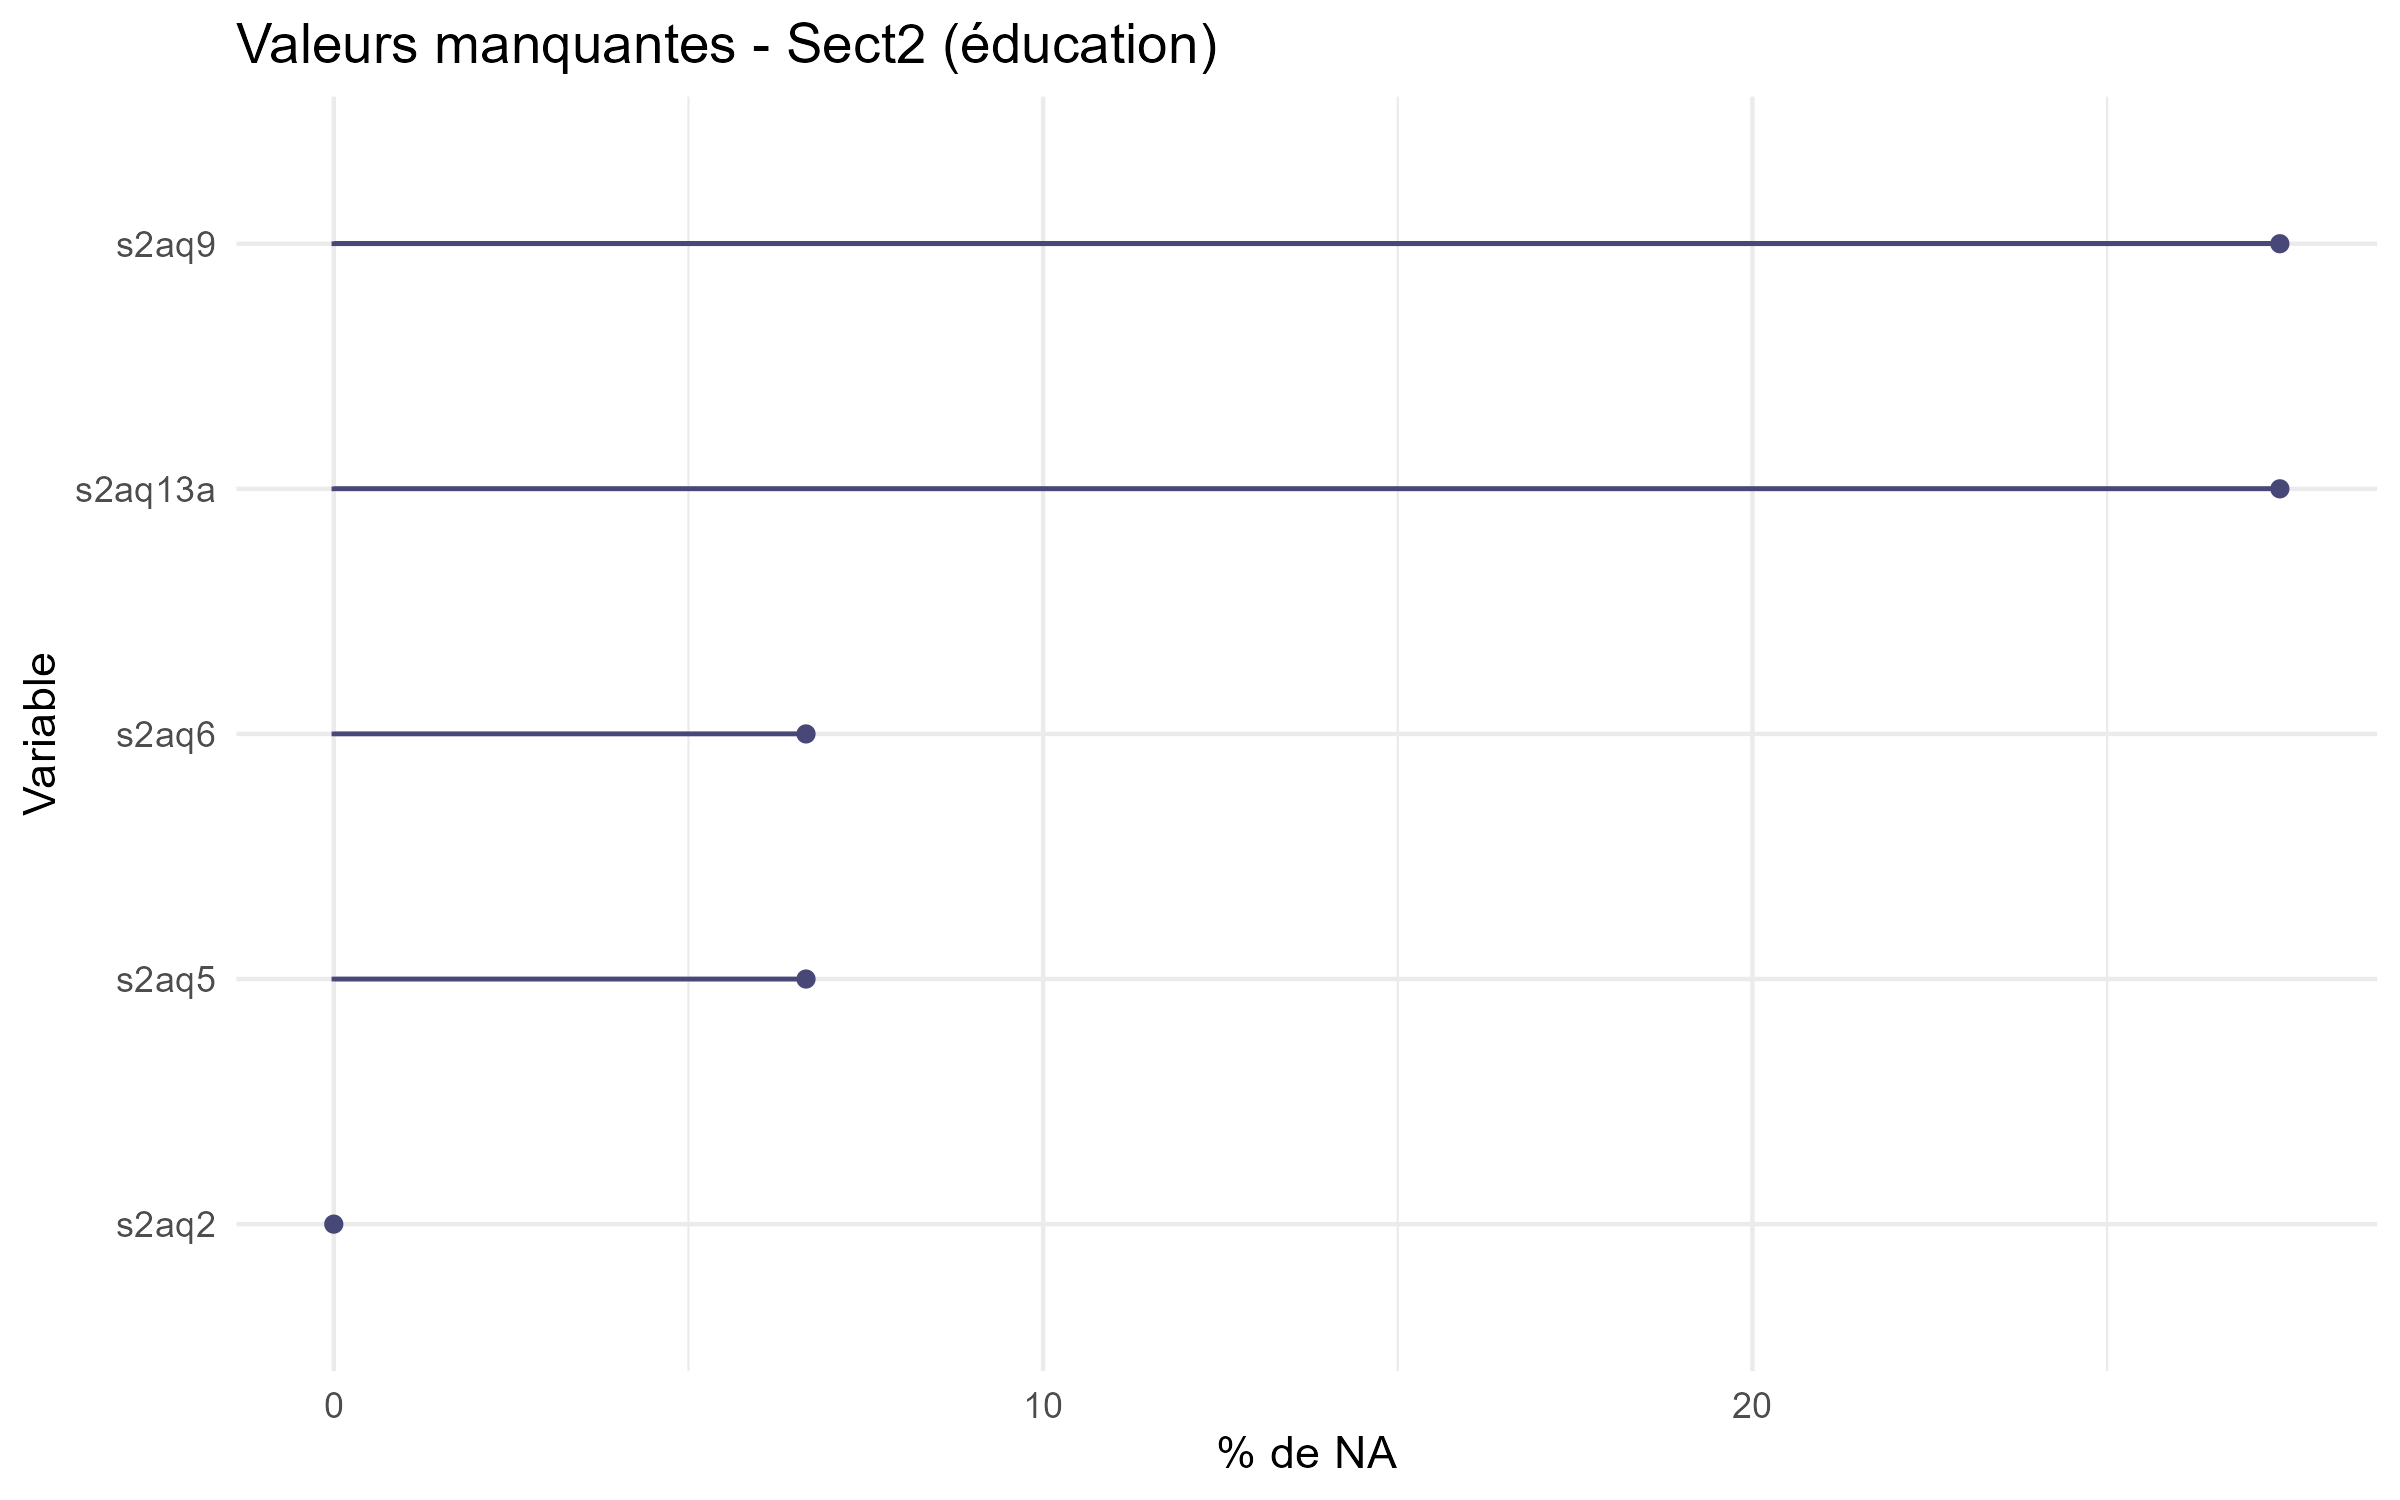
\includegraphics[width=0.95\linewidth]{../outputs/graphs/missing_sect2_tp2} 

}

\caption{Structure des valeurs manquantes dans sect2 (GHS-W4 2018) --- les blocs de 27,44\% et 64,95\% illustrent les manquants structurels du module education}\label{fig:an2_fig_missing_sect2}
\end{figure}

\subsection{Méthodes statistiques}\label{muxe9thodes-statistiques}

L'analyse bivariée mobilise des méthodes adaptées à la nature ordinale
de la variable dépendante (\texttt{niveau\_educ}). Pour les croisements
avec des variables nominales (sexe, zone), le test du \(\chi^2\) de
Pearson permet de tester l'indépendance, complété par le V de Cramér
pour quantifier la force de l'association (seuils conventionnels :
faible \textless{} 0,1 ; modérée 0,1--0,3 ; forte \textgreater{} 0,3).
La correction de Yates est appliquée pour les tables \(2 \times 2\).
Pour les comparaisons de distributions entre groupes d'âge, le test non
paramétrique de Kruskal-Wallis est préféré à l'ANOVA compte tenu de la
non-normalité de la variable, avec l'\(\eta^2\) comme mesure de taille
d'effet. Les comparaisons post-hoc sont réalisées par le test de Dunn
avec correction de Bonferroni pour contrôler l'inflation du risque de
première espèce. Les intervalles de confiance sont calculés par la
méthode de Wilson pour les proportions et de Clopper-Pearson (méthode
exacte) pour les taux de scolarisation. Le seuil de significativité
retenu est \(\alpha = 0{,}05\).

\begin{center}\rule{0.5\linewidth}{0.5pt}\end{center}

\section{Tâche 7 --- Chargement et jointure des
données}\label{tuxe2che-7-chargement-et-jointure-des-donnuxe9es}

La constitution du fichier analytique repose sur une jointure gauche
(\emph{left join}) du fichier \texttt{sect2} avec le fichier
\texttt{sect1}, réalisée sur la clé composite \texttt{(hhid,\ indiv)}
identifiant de manière unique chaque individu au sein de son ménage.
Cette approche garantit la conservation de l'intégralité des 26 557
observations de \texttt{sect2}. Le taux d'appariement obtenu est de
\textbf{100 \%}, confirmant la cohérence structurelle des deux fichiers
au sein du même millésime d'enquête.

Après application de l'algorithme de construction de
\texttt{niveau\_educ} et exclusion des valeurs manquantes non
structurelles, l'échantillon analytique se décompose comme suit :
\textbf{19 271 individus} disposent d'un niveau d'éducation documenté,
dont \textbf{10 345 adultes de 18 ans et plus} retenus pour les analyses
comparatives des tâches 9, 10 et 12, et \textbf{7 830 enfants de 6 à 17
ans} retenus pour l'analyse de scolarisation de la tâche 11. Les
\textbf{7 286 individus} restants ont été exclus pour manquants
structurels (nourrissons et enfants de moins de 5 ans).

\begin{center}\rule{0.5\linewidth}{0.5pt}\end{center}

\section{Tâche 8 --- Distribution nationale du niveau
d'éducation}\label{tuxe2che-8-distribution-nationale-du-niveau-duxe9ducation}

\subsection{Analyse descriptive}\label{analyse-descriptive}

La description de la distribution nationale du niveau d'éducation
constitue le socle de toute analyse comparative ultérieure. Elle permet
d'établir le portrait éducatif de la population nigériane à la date de
l'enquête et de situer le pays dans son contexte régional. L'analyse
porte sur les \textbf{19 271 individus} disposant d'une information
éducative exploitable, toutes tranches d'âge confondues.

La distribution révèle une nette domination du niveau \emph{Primaire},
qui concentre à lui seul \textbf{7 068 individus, soit 36,7 \%} de
l'échantillon analysable. Le niveau \emph{Senior Secondary} arrive en
deuxième position avec \textbf{4 617 individus (24,0 \%)}, suivi du
niveau \emph{Tertiaire} avec \textbf{3 595 individus (18,7 \%)}. Le
\emph{Junior Secondary} représente \textbf{2 129 individus (11,0 \%)},
et la catégorie \emph{Aucun} --- individus n'ayant jamais fréquenté une
école formelle --- concerne \textbf{1 862 individus, soit 9,7 \%} de
l'échantillon analysable.

\begin{figure}

{\centering 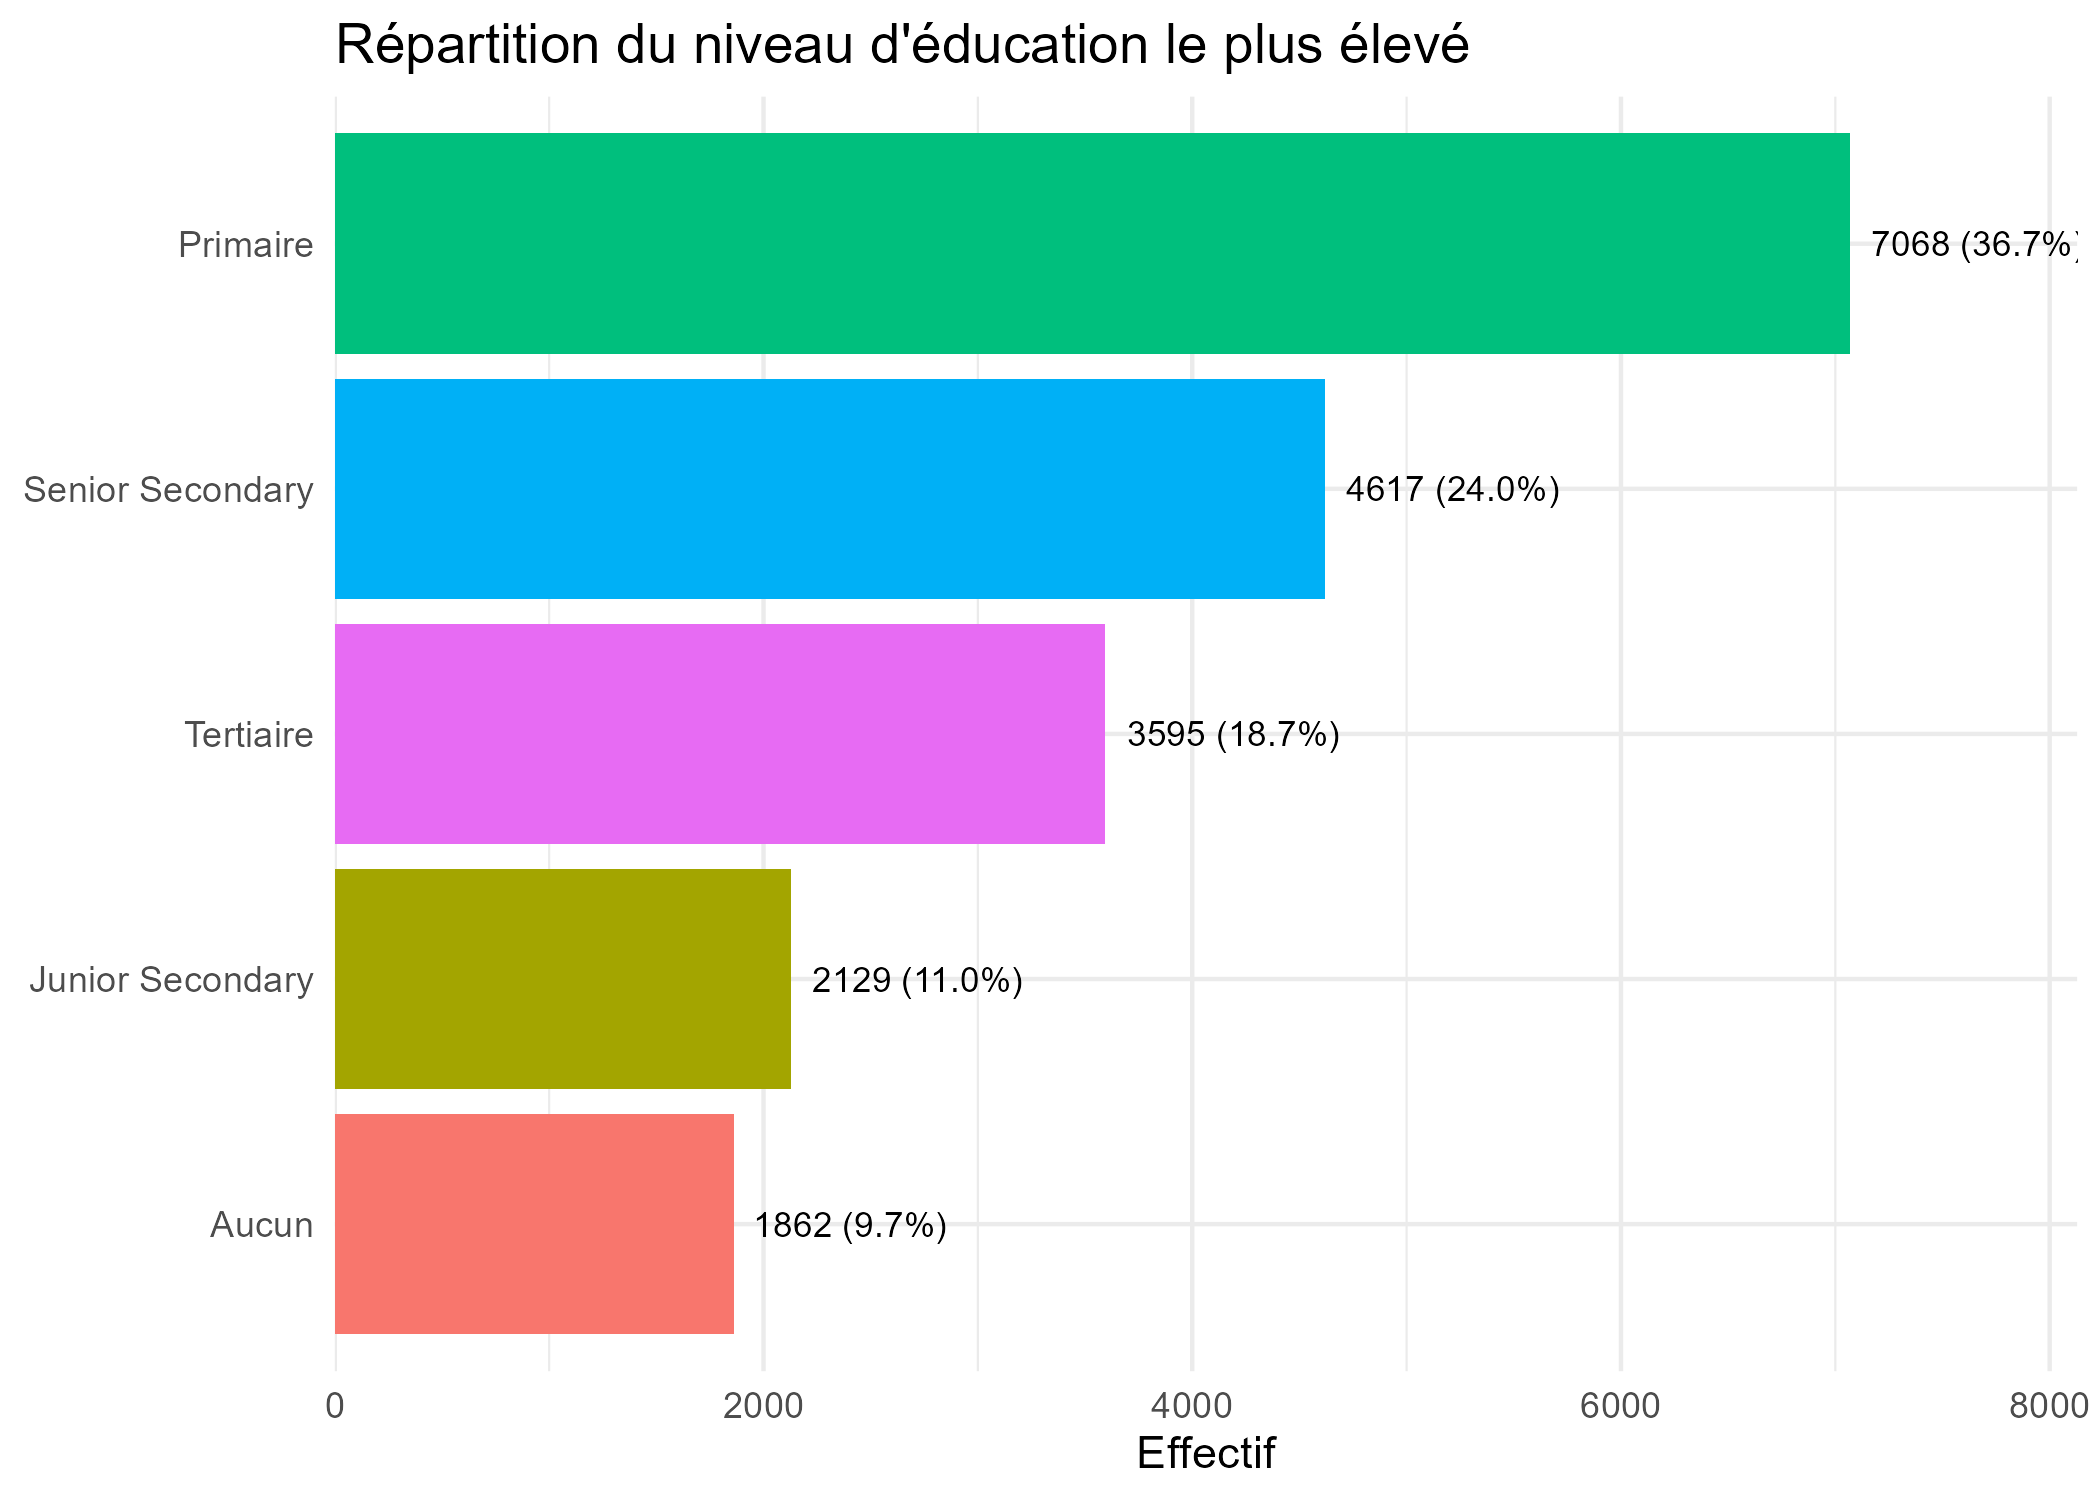
\includegraphics[width=0.95\linewidth]{../outputs/graphs/niveau_educ_barplot} 

}

\caption{Distribution du niveau d'education (N = 19 271 individus avec information disponible) --- GHS-W4 Nigeria 2018}\label{fig:an2_fig_barplot_t8}
\end{figure}

\begin{interpretbox}
\textbf{Interprétation.} La structure observée doit être lue avec prudence~: elle reflète la \textbf{composition démographique de l'échantillon} et non exclusivement le capital éducatif de la population adulte. La proportion élevée du niveau Primaire (36{,}7\,\%) s'explique en grande partie par l'inclusion des enfants et adolescents encore en cours de scolarisation, pour qui le niveau primaire est le niveau d'entrée dans le système. De même, la catégorie \textit{Aucun} (9{,}7\,\%) est mécaniquement sous-estimée dans cet échantillon global~: les enfants trop jeunes pour être scolarisés, qui seraient codés \textit{Aucun}, sont précisément ceux exclus pour manquants structurels. L'analyse par sous-population adulte (Tâche 9) et par groupe d'âge (Tâche 10) permettra de mieux isoler les dynamiques générationnelles.
\end{interpretbox}

\begin{center}\rule{0.5\linewidth}{0.5pt}\end{center}

\section{Tâche 9 --- Niveau d'éducation par
sexe}\label{tuxe2che-9-niveau-duxe9ducation-par-sexe}

\subsection{Contexte et enjeux}\label{contexte-et-enjeux}

Les inégalités éducatives de genre constituent l'une des dimensions les
plus documentées du développement humain en Afrique subsaharienne. Au
Nigeria, elles sont particulièrement marquées par des facteurs culturels
et économiques : mariages précoces, pratiques religieuses limitant la
scolarisation des filles dans certaines régions du Nord, coût
d'opportunité élevé de la scolarisation féminine dans les ménages ruraux
pauvres (Abubakar, 2020). L'analyse est restreinte aux \textbf{10 345
adultes de 18 ans et plus} --- 5 431 hommes et 4 914 femmes --- afin
d'observer des trajectoires éducatives complètes ou largement entamées.

\subsection{Distribution comparée par
sexe}\label{distribution-comparuxe9e-par-sexe}

\begin{figure}

{\centering 
\includegraphics[width=0.95\linewidth]{../outputs/graphs/education_par_sexe} 

}

\caption{Niveau d'education selon le sexe --- Adultes 18 ans et plus (N = 10 345), GHS-W4 2018}\label{fig:an2_fig_sexe_t9}
\end{figure}

Parmi les \textbf{5 431 hommes}, la répartition par niveau est la
suivante : 26 individus sans instruction (0,48 \%), 1 198 au niveau
Primaire (22,1 \%), 359 au Junior Secondary (6,6 \%), 2 158 au Senior
Secondary (39,7 \%) et 1 690 au niveau Tertiaire (31,1 \%). Parmi les
\textbf{4 914 femmes}, la distribution diffère sensiblement : 47 femmes
sans instruction (0,96 \%), 1 416 au niveau Primaire (28,8 \%), 379 au
Junior Secondary (7,7 \%), 1 687 au Senior Secondary (34,3 \%) et 1 385
au niveau Tertiaire (28,2 \%).

Ces proportions révèlent deux asymétries principales. D'une part, les
femmes sont davantage concentrées au niveau Primaire, avec un écart de
\textbf{+6,7 points} par rapport aux hommes (28,8 \% contre 22,1 \%).
D'autre part, les hommes dominent au Senior Secondary avec \textbf{+5,4
points} d'avantage (39,7 \% contre 34,3 \%). La catégorie \emph{Aucun}
est deux fois plus fréquente chez les femmes (0,96 \%) que chez les
hommes (0,48 \%).

\subsection{Test d'indépendance et mesure
d'association}\label{test-dinduxe9pendance-et-mesure-dassociation}

Le test du \(\chi^2\) de Pearson donne une statistique de
\textbf{\(\chi^2 = 87{,}09\)} avec 4 degrés de liberté et une p-value
inférieure à \(2{,}2 \times 10^{-16}\) : l'hypothèse nulle
d'indépendance entre le sexe et le niveau d'éducation est rejetée avec
une très forte certitude statistique.

\begin{interpretbox}
\textbf{Interprétation.} Cependant, la significativité statistique ne renseigne pas sur la magnitude de l'association. Le \textbf{V de Cramér de 0{,}092} classe celle-ci dans la catégorie \textbf{faible} (< 0{,}1), malgré la très haute significativité du test. Ce résultat illustre un phénomène statistique classique~: avec un large échantillon ($N = 10\,345$), même des différences substantiellement modestes génèrent des p-values infinitésimales. En termes substantiels, si des inégalités de genre existent bien, elles restent d'une ampleur limitée comparativement aux inégalités géographiques documentées dans la Tâche 12. Cette nuance est importante pour le calibrage des politiques publiques~: une intervention ciblée sur le genre sera pertinente, mais ne devra pas occulter d'autres déterminants plus puissants de l'inégalité éducative au Nigeria.
\end{interpretbox}

\begin{center}\rule{0.5\linewidth}{0.5pt}\end{center}

\section{Tâche 10 --- Niveau d'éducation par groupe
d'âge}\label{tuxe2che-10-niveau-duxe9ducation-par-groupe-duxe2ge}

\subsection{Contexte et hypothèses}\label{contexte-et-hypothuxe8ses}

L'analyse de la relation entre l'âge et le niveau d'éducation atteint
permet d'appréhender indirectement les \textbf{dynamiques
générationnelles} du système éducatif nigérian. Sous l'hypothèse d'un
progrès continu de la scolarisation, on s'attend à observer des niveaux
d'éducation plus élevés chez les cohortes les plus jeunes, qui ont
bénéficié de l'expansion du réseau scolaire public, de la gratuité de
l'enseignement primaire introduite par l'UBE Act de 2004, et des
programmes successifs d'aide à la scolarisation. Il faut néanmoins
rappeler que l'analyse reste transversale : les différences observées
confondent des effets d'âge, de période et de cohorte qui ne peuvent
être distingués sans données longitudinales.

\subsection{Distribution par groupe
d'âge}\label{distribution-par-groupe-duxe2ge}

\begin{figure}

{\centering 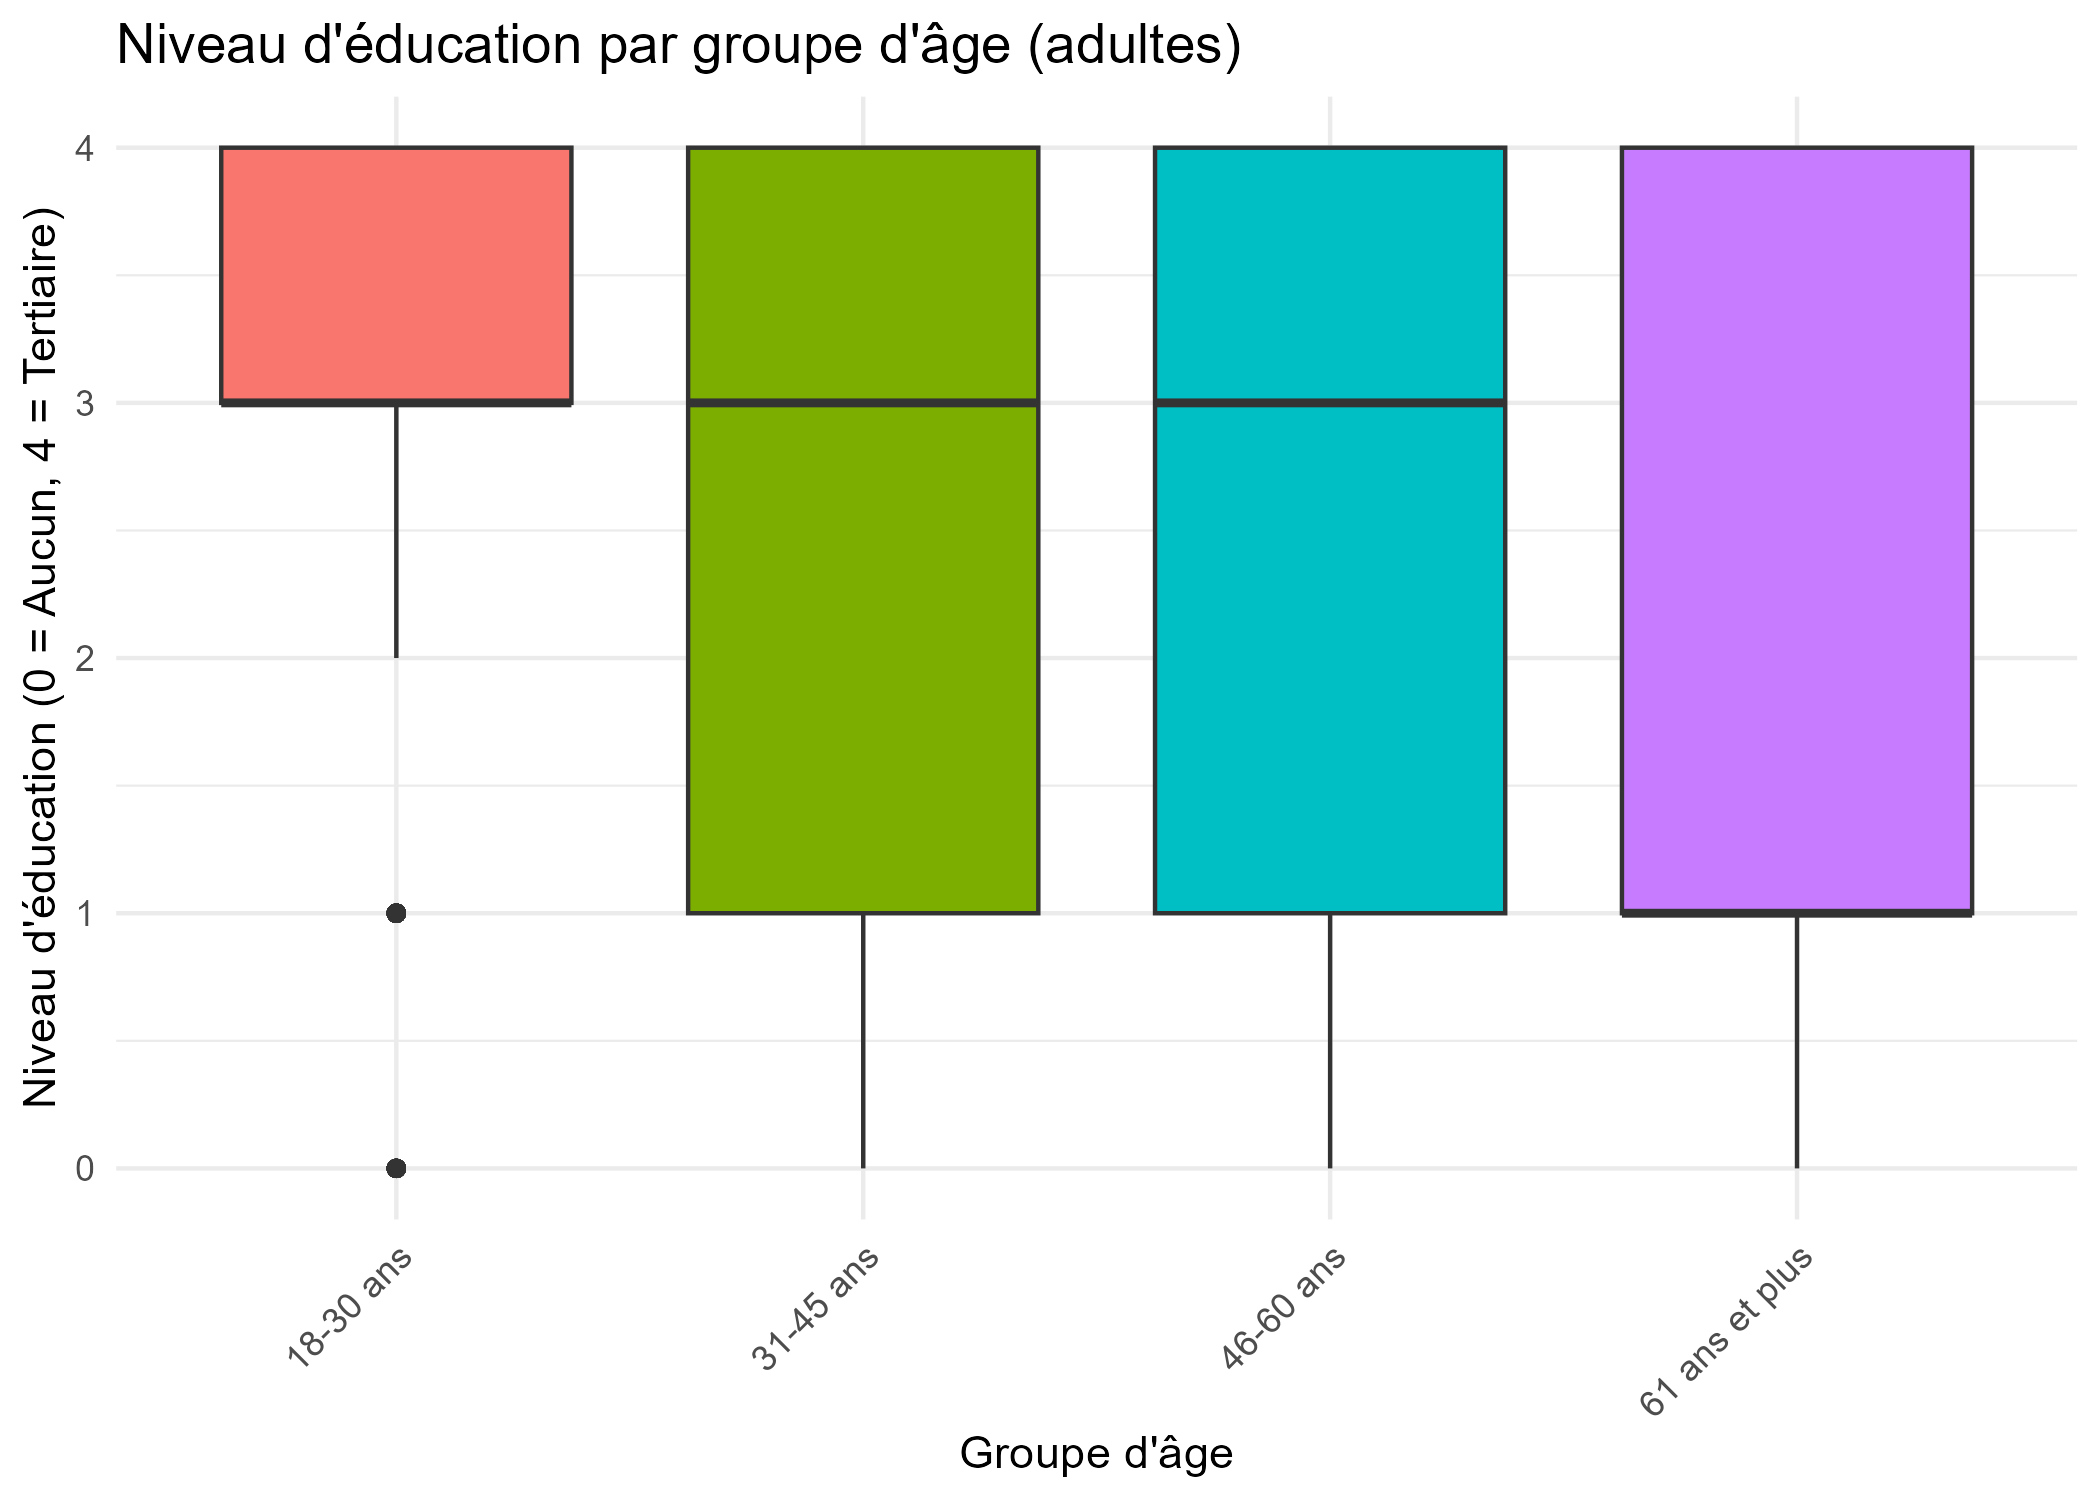
\includegraphics[width=0.95\linewidth]{../outputs/graphs/education_par_age_boxplot} 

}

\caption{Distribution du niveau d'education (score numerique 1--5) selon le groupe d'age --- Adultes 18+, GHS-W4 2018}\label{fig:an2_fig_boxplot_t10}
\end{figure}

L'échantillon adulte se répartit en quatre groupes : \textbf{4 505
individus âgés de 18 à 30 ans}, \textbf{3 149 individus de 31 à 45 ans},
\textbf{1 858 individus de 46 à 60 ans} et \textbf{833 individus de 61
ans et plus}. Les statistiques de position révèlent des profils
contrastés. Les 18--30 ans et les 31--45 ans affichent tous deux une
médiane de 3 (correspondant au Junior ou Senior Secondary), mais le
premier quartile (Q1) du groupe le plus jeune est de 3, contre 1 pour
les 31--45 ans : cela signifie que la moitié inférieure des jeunes
adultes atteint déjà le niveau secondaire, là où la moitié inférieure
des 31--45 ans reste au niveau primaire ou sans instruction. Les 46--60
ans présentent également une médiane de 3 mais avec Q1 = 1, signe d'une
dispersion interne plus forte. Le groupe des \textbf{61 ans et plus} se
distingue nettement avec une médiane à 1 (\emph{Aucun} ou
\emph{Primaire}), traduisant une période de vie où l'accès à l'école
formelle était très limité.

\subsection{Test de Kruskal-Wallis et post-hoc
Dunn}\label{test-de-kruskal-wallis-et-post-hoc-dunn}

Le test de Kruskal-Wallis confirme l'existence de différences hautement
significatives entre les quatre groupes d'âge (\textbf{H = 122\{,\}54},
3 degrés de liberté, \(p < 10^{-15}\)). La taille d'effet
\(\eta^2 = 0{,}012\) est modeste, indiquant que le groupe d'âge
n'explique qu'environ 1,2 \% de la variance dans les rangs du niveau
d'éducation.

Les comparaisons post-hoc de Dunn (correction Bonferroni) révèlent que
toutes les paires de groupes sont significativement différentes.
L'opposition la plus marquée est celle entre les \textbf{18--30 ans} et
les \textbf{61 ans et plus} (\(z = -10{,}01\), \(p < 10^{-22}\)). La
paire 18--30 vs 46--60 est également très significative
(\(z = -6{,}75\), \(p < 10^{-10}\)), tout comme 31--45 vs 61+
(\(z = -7{,}17\), \(p < 10^{-11}\)) et 46--60 vs 61+ (\(z = -4{,}59\),
\(p < 10^{-4}\)). La comparaison la moins contrastée est celle entre les
\textbf{31--45 et les 46--60 ans} (\(z = -3{,}00\), \(p = 0{,}016\)),
les deux groupes se chevauchant partiellement sur les décennies
d'expansion scolaire.

\begin{interpretbox}
\textbf{Interprétation.} Ces résultats documentent un \textbf{progrès éducatif intergénérationnel réel mais encore incomplet}. Si les jeunes adultes nigérians sont significativement mieux éduqués que leurs aînés, l'effet de génération reste de faible amplitude ($\eta^2 = 0{,}012$)~: l'expansion scolaire post-1990 a bien touché les jeunes cohortes, mais n'a pas suffi à combler l'ensemble des inégalités héritées. L'effet observé mêle par ailleurs des effets d'âge (les plus vieux ont eu moins de temps pour se scolariser), de période (amélioration des politiques éducatives) et de cohorte (conditions historiques de chaque génération), qui sont impossibles à distinguer avec une seule vague d'enquête transversale.
\end{interpretbox}

\begin{center}\rule{0.5\linewidth}{0.5pt}\end{center}

\section{Tâche 11 --- Scolarisation des 6--17 ans par
zone}\label{tuxe2che-11-scolarisation-des-617-ans-par-zone}

\subsection{Contexte et enjeux}\label{contexte-et-enjeux-1}

La scolarisation des enfants en âge d'école primaire et secondaire
inférieure (6--17 ans) est un indicateur directement lié aux objectifs
de développement durable (ODD 4 : éducation de qualité pour tous). Au
Nigeria, l'inégalité urbain-rural d'accès à l'éducation est structurelle
: les zones rurales souffrent d'un déficit chronique d'établissements
scolaires publics, d'enseignants qualifiés et de cantines scolaires
(World Bank, 2019). L'analyse porte sur les \textbf{7 830 enfants de 6 à
17 ans} présents dans l'échantillon, dont \textbf{2 315 en milieu
urbain} et \textbf{5 515 en milieu rural}.

\subsection{Résultats et indicateurs
statistiques}\label{ruxe9sultats-et-indicateurs-statistiques}

En milieu \textbf{urbain}, 2 136 enfants sont scolarisés et 179 ne le
sont pas, soit un taux de scolarisation de \textbf{92,3 \%} (IC 95 \%
Clopper-Pearson : {[}91,1 \% ; 93,3 \%{]}). En milieu \textbf{rural}, 4
880 enfants sont scolarisés et 635 ne le sont pas, soit un taux de
\textbf{88,5 \%} (IC 95 \% : {[}87,6 \% ; 89,3 \%{]}). La différence
absolue est de \textbf{+3,8 points} en faveur du milieu urbain, et le
risque relatif de \textbf{1,043} signifie qu'un enfant urbain a une
probabilité 4,3 \% supérieure d'être scolarisé qu'un enfant rural.

Le test du \(\chi^2\) avec correction de Yates donne
\textbf{\(\chi^2 = 24{,}63\)} (\(p = 6{,}94 \times 10^{-7}\)),
confirmant que cet écart est hautement significatif et non imputable à
la variabilité d'échantillonnage.

\begin{figure}

{\centering 
\includegraphics[width=0.95\linewidth]{../outputs/graphs/taux_scolarisation_par_zone_detail} 

}

\caption{Taux de scolarisation des enfants de 6--17 ans par zone de residence, avec intervalles de confiance a 95\% (methode Clopper-Pearson) --- GHS-W4 Nigeria 2018}\label{fig:an2_fig_scol_t11}
\end{figure}

\begin{interpretbox}
\textbf{Interprétation.} L'écart de 3{,}8 points, bien que modeste en valeur relative, représente en termes absolus une part non négligeable de la population enfantine. Les deux intervalles de confiance à 95\,\% ne se chevauchent pas, attestant d'une différence réelle entre les deux zones. Ces résultats militent pour un renforcement prioritaire des infrastructures scolaires en milieu rural~: construction de salles de classe, déploiement d'enseignants qualifiés dans les zones enclavées, adaptation du calendrier scolaire aux cycles agricoles. Une attention particulière doit être portée aux filles rurales, qui cumulent les désavantages de genre et de territoire.
\end{interpretbox}

\begin{center}\rule{0.5\linewidth}{0.5pt}\end{center}

\section{Tâche 12 --- Taux de sans-instruction par
État}\label{tuxe2che-12-taux-de-sans-instruction-par-uxe9tat}

\subsection{Contexte géographique}\label{contexte-guxe9ographique}

La décomposition géographique des inégalités éducatives au niveau
étatique est cruciale pour le ciblage des politiques publiques dans un
État fédéral comme le Nigeria, où les gouvernements des États disposent
d'une large autonomie en matière d'éducation. La littérature distingue
classiquement un clivage Nord-Sud structuré par des facteurs historiques
(implantation des missions chrétiennes au Sud, prédominance de
l'éducation coranique au Nord), économiques (inégalités de revenus et
d'infrastructures) et sécuritaires (insurrection de Boko Haram dans le
Nord-Est depuis 2009, ayant provoqué la fermeture de milliers d'écoles).
L'indicateur retenu est le \textbf{taux de sans-instruction}, défini
comme la proportion d'individus classés dans la catégorie \emph{Aucun}
parmi ceux disposant d'une information éducative.

\subsection{Profils extrêmes}\label{profils-extruxeames}

Les contrastes inter-étatiques sont saisissants. À une extrémité du
spectre, \textbf{Kebbi} (Nord-Ouest) affiche le taux le plus élevé avec
\textbf{67,8 \%} (162 sans-instruction sur 239 individus) : près de 7
individus sur 10 n'ont jamais fréquenté une école formelle. Viennent
ensuite \textbf{Niger} (55,6 \%, soit 210 sur 378), \textbf{Bauchi}
(46,3 \%, soit 321 sur 694), \textbf{Yobe} (43,2 \%, soit 89 sur 206) et
\textbf{Taraba} (39,8 \%, soit 141 sur 354). Ces cinq États
appartiennent tous au Nord géographique.

À l'opposé, \textbf{Rivers} (Sud-Sud) enregistre le taux le plus bas
avec seulement \textbf{2,1 \%} (6 sans-instruction sur 287), suivi de
\textbf{Lagos} (4,7 \%, soit 27 sur 569), \textbf{Bayelsa} (6,7 \%, soit
11 sur 163), \textbf{Abia} (6,9 \%, soit 43 sur 625) et \textbf{Akwa
Ibom} (8,5 \%, soit 51 sur 597). Ces cinq États sont tous situés dans la
frange côtière et le Sud-Sud du pays.

L'écart maximal entre Rivers (2,1 \%) et Kebbi (67,8 \%) atteint
\textbf{65,7 points de pourcentage}, traduisant des trajectoires
éducatives radicalement divergentes au sein d'un même pays.

\subsection{Carte choroplèthe}\label{carte-choropluxe8the}

\begin{figure}

{\centering 
\includegraphics[width=0.92\linewidth]{../outputs/graphs/carte_taux_sans_instruction_avec_noms} 

}

\caption{Carte choroplethe du taux de sans-instruction par Etat nigerian --- GHS-W4 2018. Gradient du blanc (taux faible) au rouge fonce (taux eleve).}\label{fig:an2_fig_carte_t12}
\end{figure}

\begin{interpretbox}
\textbf{Interprétation.} La carte confirme et spatialise le \textbf{clivage Nord-Sud} avec une précision qui dépasse la simple dichotomie régionale. Le gradient de couleur met en évidence un pôle de forte déprivation éducative dans le Nord-Ouest (Kebbi 67{,}8\,\%, Niger 55{,}6\,\%, Katsina 37{,}7\,\%, Kwara 33{,}2\,\%) et le Nord-Est (Bauchi 46{,}3\,\%, Taraba 39{,}8\,\%, Gombe 21{,}1\,\%), des niveaux intermédiaires dans la « Middle Belt » (Plateau 36{,}7\,\%, Benue 24{,}6\,\%, Kaduna 25{,}3\,\%), et un pôle de relative bonne performance dans le Sud (Rivers 2{,}1\,\%, Lagos 4{,}7\,\%, Bayelsa 6{,}7\,\%). Ce gradient correspond étroitement à la carte des investissements historiques en infrastructure scolaire~: les États du Sud, ayant bénéficié dès la période coloniale de l'implantation d'établissements missionnaires, ont développé une tradition scolaire profondément ancrée. La situation du Nord-Est est exacerbée par l'insurrection de Boko Haram, qui a provoqué depuis 2009 la destruction ou fermeture d'un grand nombre d'établissements scolaires dans les États de Bauchi et Yobe notamment.
\end{interpretbox}

\begin{center}\rule{0.5\linewidth}{0.5pt}\end{center}

\section{Synthèse et
recommandations}\label{synthuxe8se-et-recommandations}

\subsection{Synthèse des résultats}\label{synthuxe8se-des-ruxe9sultats}

L'ensemble des analyses conduit à un tableau cohérent des inégalités
éducatives au Nigeria en 2018. La Tâche 8 révèle que, parmi les
individus disposant d'une information éducative, le niveau
\emph{Primaire} est dominant (36,7 \%) et que la catégorie \emph{Aucun}
ne représente que 9,7 \% --- un chiffre qui sous-estime toutefois la
réalité adulte, compte tenu de la composition de l'échantillon. La Tâche
9 montre que si une inégalité de genre existe bien (\(\chi^2 = 87{,}1\),
\(p < 10^{-15}\)), son amplitude reste faible (V de Cramér = 0,092) :
les femmes sont sur-représentées au Primaire (+6,7 pts) et
sous-représentées au Senior Secondary (-5,4 pts), mais les distributions
restent proches. La Tâche 10 documente un progrès éducatif
intergénérationnel réel (\(H = 122{,}5\), \(p < 10^{-15}\)) : les 18--30
ans sont significativement mieux éduqués que toutes les cohortes plus
âgées, la différence la plus marquée opposant les jeunes adultes aux 61
ans et plus (\(z = -10{,}01\)). La Tâche 11 confirme une fracture
urbain-rural significative dans la scolarisation des enfants
(\(\chi^2 = 24{,}6\), \(p < 10^{-6}\)) : 92,3 \% en urbain contre 88,5
\% en rural, soit 3,8 points d'écart. Enfin, la Tâche 12 révèle les
inégalités les plus profondes : un écart inter-étatique de 65,7 points
entre Rivers (2,1 \%) et Kebbi (67,8 \%), structuré par un clivage
géographique Nord-Sud net.

\subsection{Recommandations}\label{recommandations}

\textbf{1. Accélération de la transition Primaire → Secondaire.} Avec
36,7 \% de la population au niveau Primaire, le principal goulet
d'étranglement n'est plus l'entrée à l'école primaire mais la rétention
jusqu'au secondaire. Des bourses conditionnelles à la présence scolaire,
la gratuité des manuels au collège et un suivi individualisé des risques
d'abandon permettraient d'augmenter significativement le flux vers le
secondaire.

\textbf{2. Réduction des inégalités de genre au niveau secondaire et
supérieur.} Les leviers recommandés incluent les internats féminins en
zone rurale, le recrutement prioritaire d'enseignantes dans les États du
Nord, et les programmes de sensibilisation des familles sur la
rentabilité économique de la scolarisation des filles.

\textbf{3. Rattrapage éducatif des générations antérieures à 1990.}
L'écart générationnel documenté en Tâche 10 (\(z = -10{,}01\), groupe
18--30 vs 61+) confirme qu'une génération entière n'a pas bénéficié de
l'expansion scolaire post-1990. Des programmes d'alphabétisation
fonctionnelle des adultes, articulés à des formations professionnelles
qualifiantes, permettraient de valoriser ce capital humain
sous-exploité.

\textbf{4. Investissement différencié en milieu rural.} L'écart de 3,8
points sur le taux de scolarisation est statistiquement solide et
géographiquement concentré. L'électrification des écoles rurales,
l'adaptation du calendrier scolaire aux cycles agricoles et le
déploiement d'enseignants contractuels locaux constituent des leviers à
coût limité et à fort impact potentiel.

\textbf{5. Ciblage géographique d'urgence dans le Nord.} L'écart
inter-étatique de 65,7 points impose une réponse concentrée sur les
États du quintile le plus défavorisé --- Kebbi, Niger, Bauchi, Yobe,
Taraba. Cette réponse doit combiner reconstruction et sécurisation des
infrastructures scolaires, recrutement massif d'enseignants locaux, et
programmes de cantines scolaires pour lever les contraintes
d'opportunité pesant sur les familles.

\subsection{Limites}\label{limites}

\begin{alertbox}
\textbf{Limites.} (1) Pondérations de sondage non appliquées~: les résultats sont valides pour l'échantillon mais ne peuvent être directement extrapolés à la population nationale. (2) Analyse transversale~: effets d'âge, de période et de cohorte non distingués --- l'effet générationnel observé (T10) mêle ces trois composantes. (3) Les taux d'analphabétisme par État (T12) portent sur l'ensemble des répondants avec information disponible, et non exclusivement sur les adultes~: ils doivent être interprétés avec prudence. (4) Possible biais de sélection~: les ménages les plus défavorisés ou nomades peuvent être sous-représentés.
\end{alertbox}

\begin{center}\rule{0.5\linewidth}{0.5pt}\end{center}

\vfill

\emph{Rapport produit dans le cadre du cours
\textbf{Projet statistique sous R et Python}}

\emph{Superviseur\textasciitilde: \textbf{Aboubacar HEMA} \textbar{}
ENSAE Pierre Ndiaye, Dakar, Sénégal}

\emph{Auteurs\textasciitilde: \textbf{Agnangma Sanam David Landry} \&
\textbf{Cheikh Thioub} \textbar{} ISE 1 \textbar{} 2025--2026}

\emph{Données\textasciitilde: Nigeria General Household Survey --- Wave
4 (2018) \textbar{} World Bank / NBS Nigeria} ```

\end{document}
